\newpage
\section{Discontinuous Galerkin Method}

The Discontinuous Galerkin Method is a method of resolving differential equations through a mesh. It is similar to the Finite Element Method and the Finite Volume Method. This section is for the reader with a beginner's understanding of the Finite Element Method.

\subsection{Basic Overview}


\begin{figure}[ht]
\centering
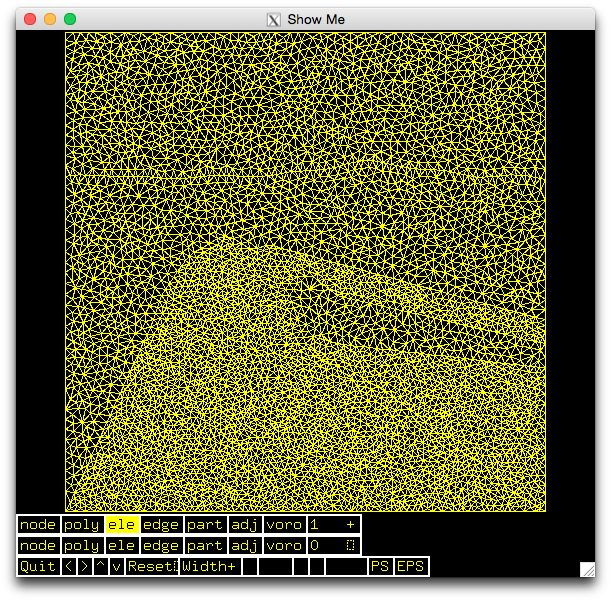
\includegraphics[width=0.7\textwidth]{Images/Example-Mesh.png}
\caption{Example Mesh used to cover example data}
\label{fig:couches5-mesh}
\end{figure}

"Solving differential equations" (such as the acoustic wave equation) is a term that is commonly thrown around without much attention to the essential components in numerical analysis. For the common case, it means: \textbf{given a domain} (for example $[0,10]$ in one dimension or the unit sphere in three dimensions), we \textbf{take a mesh} (set of segments, triangles, tetrahedrons, etc) that covers the domain, and find the values of the variable we are solving for at \textbf{certain moments in time} and at \textbf{certain points in the domain} that are determined by the mesh.

The Discontinuous Galerkin Method is a method to "solve differential equations". It can be considered a combination of Finite Element Methods (Continuous Galerkin) and Finite Volume Methods. In other words, Discontinuous Galerkin methods are finite element methods that use discontinuous basis functions, thus acquiring more robustness for discontinuous processes. Like the Finite Volume Methods, Discontinuous Galerkin methods calculate surface integrals and fluxes of discontinuous terms.

\subsection{Basis Functions}

In Discontinuous Galerkin Methods, we can raise the accuracy of our solution by increasing the order of the polynomials that approximate it. 

The way we represent our solution to the differential equation, is a group of polynomials for each element in the mesh; each polynomial takes a value of $1$ at a certain point and $0$ at all the other points defined in the element. This way, when we define the solution as the linear combination of those functions, we can easily determine the value at each node from the coefficients in front of each function.

For reference, let us use as an example the 2-dimensional reference element. The nodes are as shown:




INCLUDE IMAGE HERE


Given an order $p$, the specific nodes are defined as:

$(\hat{x_i}, \hat{y_j}, \hat{y_k}) = \left( \frac{i}{p}, \frac{j}{p}, \frac{k}{p} \right)$ for each 

each element has a group of polynomials of a certain order defined on it. Those polynomials are defined such that, for certain nodes.


\subsection{Decomposing u(x,t)}

We can decompose 

\subsection{Random Thoughts to be organized later}

We can decompose u(x,t) into discontinuous space-dependent parts and time dependent parts. We let $u(x,t) = c_1(t) \phi_1(x) + c_2(t) \phi_2(x) + \ldots + c_n(t) \phi_n(x)$. 

With this method, we can then transform the equations into a linear matrix form. For example, take the term $\int_K \frac{\partial^2 u(x,t)}{\partial t^2} v(x,t) dV$.

$$\int_K \frac{\partial^2 u(x,t)}{\partial t^2} v(x,t) dV$$

We want the equalities to be satisfied for any $v(x,t)$ in our function space, so we just need to make sure that the equalities are satisfied for $v(x,t) = \phi_i(x)$ for all $i$. We can do this by using vector and matrix operations to represent multiple equations.


$$\begin{bmatrix}
\int u(x,t) \phi_1 dV \\
\int u(x,t) \phi_2 dV \\
\ldots \\
\int u(x,t) \phi_n dV
\end{bmatrix}$$

$$= \begin{bmatrix}
\int \frac{\partial^2 c_1(t)}{\partial t^2} \phi_1 \phi_1 dV \\
\int \frac{\partial^2 c_2(t)}{\partial t^2} \phi_1 \phi_2 dV \\
\ldots \\
\int \frac{\partial^2 c_n(t)}{\partial t^2} \phi_1 \phi_n dV
\end{bmatrix}$$

$$= \begin{bmatrix}
    \int \phi_1 \phi_1 dV & \int \phi_1 \phi_2 dV & \int \phi_1 \phi_3 dV & \ldots \\
    \int \phi_2 \phi_1 dV & \int \phi_2 \phi_2 dV & \int \phi_2 \phi_3 dV & \ldots \\
    \int \phi_3 \phi_1 dV & \int \phi_3 \phi_2 dV & \int \phi_3 \phi_3 dV & \ldots \\
    \ldots & \ldots & \ldots & \ldots 
\end{bmatrix} 
\frac{\partial^2}{\partial t^2} 
\begin{bmatrix}
    c_1(t) \\
    c_2(t) \\
    c_3(t) \\
    \ldots
\end{bmatrix} $$

$$= M \frac{\partial^2}{\partial t^2} U_h$$
where $M$ is the Mass matrix and $U_h$ is the vector of coefficients defining $u(x,t)$


